\documentclass[11pt]{article}
\usepackage{udec-pset}
\guia{2}{Campo Eléctrico}

\definecolor{myred}{RGB}{200,50,50}
\definecolor{myblue}{RGB}{50,50,200}
\definecolor{mygreen}{RGB}{50,150,50}

\mostrarSoluciones

\begin{document}
\crearEncabezado

\section*{Recordatorio}

\begin{boxTeoria}{Campo Eléctrico debido a Carga Puntual}
    Si tenemos una carga fuente $Q$, el campo que genera sobre un punto
    $P$ es:
    \begin{equation*}
        \vec{E} = \frac{1}{4\pi\epsilon_0} \frac{Q}{|\vec{R}|^2} \hat{R}
    \end{equation*}

    Donde:
    \begin{itemize}
        \item $\vec{R} = \vec{r}_P - \vec{r}_Q$
    \end{itemize}
\end{boxTeoria}

\begin{problema}[Distribución de Carga Lineal]
    Considere un hilo delgado en forma de semicircunferencia de radio $R$ cargado con una densidad de carga lineal uniforme $\lambda$. Este sitúa su centro el origen. Determine, el vector campo eléctrico $\vec{E}$ generado por esta distribución en el punto $P$ ubicado en el origen.

    \begin{center}
        \shorthandoff{>}
        \begin{tikzpicture}[scale=2, >=stealth]
            \draw[->, thin, gray] (-1.3, 0) -- (1.3, 0) node[right, black, scale=0.7] {$x$};
            \draw[->, thin, gray] (0, -0.2) -- (0, 1.3) node[above, black, scale=0.7] {$y$};

            \draw[ultra thick, UdeCPrincipal] (1,0) arc (0:180:1);

            \filldraw[black] (0,0) circle (1.2pt) node[below left, scale=0.8] {$P$};

            \draw[dashed, red, thick] (0,0) -- (45:1) node[midway, above left, scale=0.8] {$R$};

            \node[UdeCPrincipal, scale=0.9] at (135:1.2) {$\lambda$};
        \end{tikzpicture}
        \shorthandon{>}
    \end{center}
\end{problema}

\begin{solucion}
    Existen dos formas de abordar este ejercicio, primero es parametrizando la curva correspondiente llegando a: $\vec{r}_C(\theta) = R\cos(\theta)\hat{x} + R\sin(\theta)\hat{y}$, con intervalos $\theta\in[0, \pi]$ y diferencial de línea de $dl = Rd\theta$ y construir el diferencial de campo eléctrico.
    \\ \\
    La segunda forma se puede realizar aprovechándonos de la simetría del sistema, y es que, notamos que la componente $x$ del campo eléctrico será nula ya que cada carga ubicada a la izquierda compensa el campo formado por su asociada a la derecha. De esto rescatamos que: $d\vec{E} = dE_x\hat{x} + dE_y\hat{y}$ y $dE_x\hat{x} = 0$.
    \\ \\
    Lo siguiente es que notamos que cada elemento infinitesimal de la curva produce exactamente la misma \textbf{magnitud} de campo eléctrico sobre el punto $P$ al ubicarse a la misma distancia de este. Esta magnitud estará dada por:\\[-15pt]
    \begin{equation}
        dE = \frac{1}{4\pi\epsilon_0} \frac{dq}{R^2}
    \end{equation}
    donde $dq = \lambda dl$ y notamos además que $dl$ se puede expresar como $Rd\theta$ con $\theta\in[0, \pi]$ y $R$ el radio de la semicirunferencia.
    \\ \\
    De esta expresión nos interesa únicamente la componente $y$ del diferencial de campo $d\vec{E}$, el cual mediante la siguiente figura, se llega a que se puede extraer como: $dE_y\hat{y} = -\sin(\theta)dE\hat{y}$.

    \begin{center}
        \shorthandoff{>}
        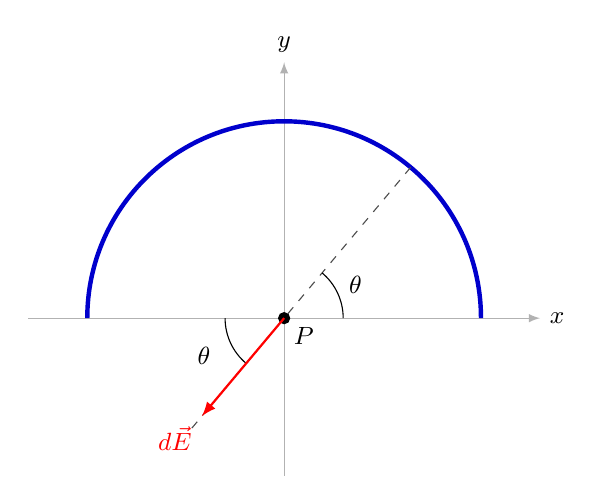
\begin{tikzpicture}[scale=2.5, font=\small]

            % --- Ejes de Coordenadas ---
            \draw[arrows={-latex}, thin, gray!60] (-1.3, 0) -- (1.3, 0) node[right, black] {$x$};
            \draw[arrows={-latex}, thin, gray!60] (0, -0.8) -- (0, 1.3) node[above, black] {$y$};

            % --- El Semicírculo ---
            \draw[ultra thick, blue!80!black] (1,0) arc (0:180:1);

            % Punto P movido a la derecha
            \filldraw[black] (0,0) circle (0.8pt);
            \node[below right] at (0,0) {$P$};

            % --- Geometría de Ángulos Opuestos por el Vértice ---
            % Línea que conecta el diferencial arriba con la dirección del campo abajo
            \draw[dashed, black!70] (50:1) -- (230:0.75);

            % Ángulo theta arriba (respecto al eje x positivo)
            \draw[thin] (0.3, 0) arc (0:50:0.3);
            \node at (25:0.4) {$\theta$};

            % Ángulo theta abajo (respecto al eje x negativo)
            % Se dibuja desde 180 (eje -x) hacia 230 (180+50)
            \draw[thin] (-0.3, 0) arc (180:230:0.3);
            \node at (205:0.45) {$\theta$};

            % --- Vector de Campo Resultante dE ---
            \draw[arrows={-latex}, thick, red] (0,0) -- (230:0.65) node[below left] {$d\vec{E}$};

        \end{tikzpicture}
        \shorthandon{>}
    \end{center}

    Finalmente sumando todos estos elementos se llega al vector de campo eléctrico total sobre $P$.

    \begin{equation}
        \vec{E} = \int_S d\vec{E} = \int_{0}^{\pi} \frac{\lambda}{4\pi\epsilon_0}\frac{-\sin{\theta}}{R^2}R\,d\theta \hat{y}
    \end{equation}

    \begin{equation}
        \vec{E} = -\frac{\lambda}{2\pi R\epsilon_0}\hat{y}
    \end{equation}

\end{solucion}

\begin{problema}[Distribución de Carga Superficial]

    Considere un plano infinito que coincide con el plano $xy$ ($z = 0$), el cual posee una densidad de carga superficial uniforme $\sigma$. Exprese la integral que permite calcular la magnitud del campo eléctrico que esta ejerce sobre una carga ubicada en $P=h\hat{z}$.
\end{problema}

\begin{solucion}
    Primero, mediante coordenadas rectangulares vemos que todo punto del plano está ubicado en la superficie: $S: \vec{r}_S(x, y) = l\hat{x} + w\hat{y}$, con $x\in[-\infty, \infty]$, $y\in[-\infty, \infty]$.
    \\
    Por lo tanto, el vector separación entre el elemento diferencial del plano y el punto de interés es: $\vec{R} = \vec{r}_P - \vec{r}_S = h\hat{z} - l\hat{x} - w\hat{y}$
    \\
    La carga asociada a este elemento del plano está dada por: $dq = \sigma dS$, donde $dS = dldw$, así, el campo eléctrico ejercido por el plano hacia el punto $P$ es:
    \begin{equation}
        d\vec{E} = \frac{1}{4\pi\epsilon_0}\frac{dq}{|\vec{R}|^2}\hat{R}
    \end{equation}

    \begin{align}
        d\vec{E} = \frac{1}{4\pi\epsilon_0}\frac{\sigma}{|\vec{R}|^3}\vec{R}\,dldw
        \\
        d\vec{E} = \frac{\sigma}{4\pi\epsilon_0}\frac{h\hat{z} - l\hat{x} - w\hat{y}}{\sqrt{h^2+l^2+w^2}^3}\,dldw
    \end{align}

    Finalmente, sumando todos estos aportes, obtendremos el campo eléctrico total sobre el punto.

    \begin{equation}
        \vec{E} = \int_S d\vec{E} = \int_{-\infty}^{\infty} \int_{-\infty}^{\infty}\frac{\sigma}{4\pi\epsilon_0}\frac{h\hat{z} - l\hat{x} - w\hat{y}}{\sqrt{h^2+l^2+w^2}^3}\,dldw
    \end{equation}

    Notamos que por simetría las componentes laterales debiesen anularse por completo entre sí, únicamente la componente vertical. Por lo tanto la expresión resultante es:

    \begin{equation}
        \vec{E} = \int_S d\vec{E} = \frac{h\sigma}{4\pi\epsilon_0} \int_{-\infty}^{\infty} \int_{-\infty}^{\infty} \frac{1}{\sqrt{h^2+l^2+w^2}^3}\,dldw\,\hat{z}
    \end{equation}

\end{solucion}

\begin{problema}[Distribución de Carga Volumétrica]
    Una esfera sólida de radio $a$ posee una densidad de carga volumétrica no uniforme definida por:

    \begin{equation*}
        \rho(r) = \rho_0 \left( \frac{r - a}{a} \right)
    \end{equation*}

    donde $r$ es la distancia radial desde el centro de la esfera. Encontrar la intensidad del campo eléctrico en un punto situado a una distancia $R$ muy grande ($R \gg a$). ¿Qué cosas deben asumirse?
\end{problema}

\begin{solucion}
    Debido a que el punto que nos interesa calcular la intensidad de campo eléctrico esta muy alejado de la esfera, nos podemos ayudar de tratar a la carga total de la esfera como una \textbf{Carga Puntual} ejerciendo fuerza sobre este punto a distancia $R$.
    \\ \\
    De esta forma lo único que necesitamos es obtener la carga total de la esfera y calcular la intensidad de campo eléctrico que ejerce sobre este punto de interés.
    \\ \\
    Sabemos que $dq = \rho dV$, pero además que $\rho$ varía en base a la distancia desde el centro de la esfera según la expresión dada, por lo tanto:

    \begin{equation}
        dq = \rho(r)dV
    \end{equation}

    Luego para obtener una expresión para $dV$ en base a $r$ existen varias formas, una de ellas es que podemos tomar la superficie de una efera de radio $r$ (con $r\in[0, a]$) y multiplicarla por un pequeño grosor $r$, así:

    \begin{equation}
        dV = 4\pi r^2 dr
    \end{equation}

    Esto juntando con la expresión de $dq$ obtenemos

    \begin{equation}
        dq = \rho_0 \left( \frac{r - a}{a} \right) 4\pi r^2 dr, \qquad \text{con } r\in[0, a]
    \end{equation}

    Finalmente obtenemos la carga total de la esfera.

    \begin{align}
        Q_S = \int_S dq = \int_{0}^{a} \rho_0 \left( \frac{r - a}{a} \right)4\pi r^2 \,dr
        \\
        Q_S = \frac{4\pi\rho_0}{a} \int_{0}^{a} r^3-ar^2\,dr
    \end{align}

    \begin{align}
        Q_S = \frac{4\pi\rho_0}{a} \left.\left(\frac{r^4}{4}-a\frac{r^3}{3}\right)\right|_0^a
        \\
        Q_S = -\frac{a^3\pi\rho_0}{3}
    \end{align}

    Finalmente, la magnitud de campo eléctrico que ejerce esta esfera sobre el punto a una distancia $R$ muy lejana es:

    \begin{align}
        E = \left|\frac{1}{4\pi\epsilon_0} \frac{Q_S}{R^2}\right|
        \\
        E = \left|\frac{1}{4\pi\epsilon_0} \frac{-\frac{a^3\pi\rho_0}{3}}{R^2}\right|
        \\
        E = \frac{a^3\rho_0}{12R^2\epsilon_0}
    \end{align}
\end{solucion}


\end{document}